In this section, we introduce some details about the food datasets and the two architectures used for our experiments.
\subsection{Models}
In this paper, AlexNet and GoogLeNet are their Caffe \cite{jia2014caffe} implementation and all the results for a specific CNN architecture are obtained from single model.

\textbf{AlexNet}
 contains 5 layers followed by the auxiliary classifier which contains 2 fully connected layers (FC) and 1 softmax layer. Each of the first two layers can be subdivided into 3 components: convolutional layer with rectified linear units (ReLUs), local response normalization layer (LRN) and max pooling layer. Layer 3 and layer 4 contain just convolutional layer with ReLUs while layer 5 is similar to the first two layers except for the LRN. For each of the fully connected layer, 1 ReLUs and 1 dropout \cite{srivastava2014dropout} layer are followed.

 \textbf{GoogLeNet}
  shows another trend of deep CNN architecture with lots of small receptive fields. Figure \ref{incept} shows the architecture a inception cell. Inspired by \cite{linNiN}, lots of $1\times 1$ convolutional layers are used for computational efficiency. Another interesting feature of GoogLeNet is that there are two extra auxiliary classifiers in intermediate layers. During the training procedure, the loss of these two classifiers are counted into the total loss with a discount weight 0.3, in addition with the loss of the classifier on top. More architecture details can be found from \cite{szegedy2014going}.

\begin{figure}
  \centering
  % Requires \usepackage{graphicx}
  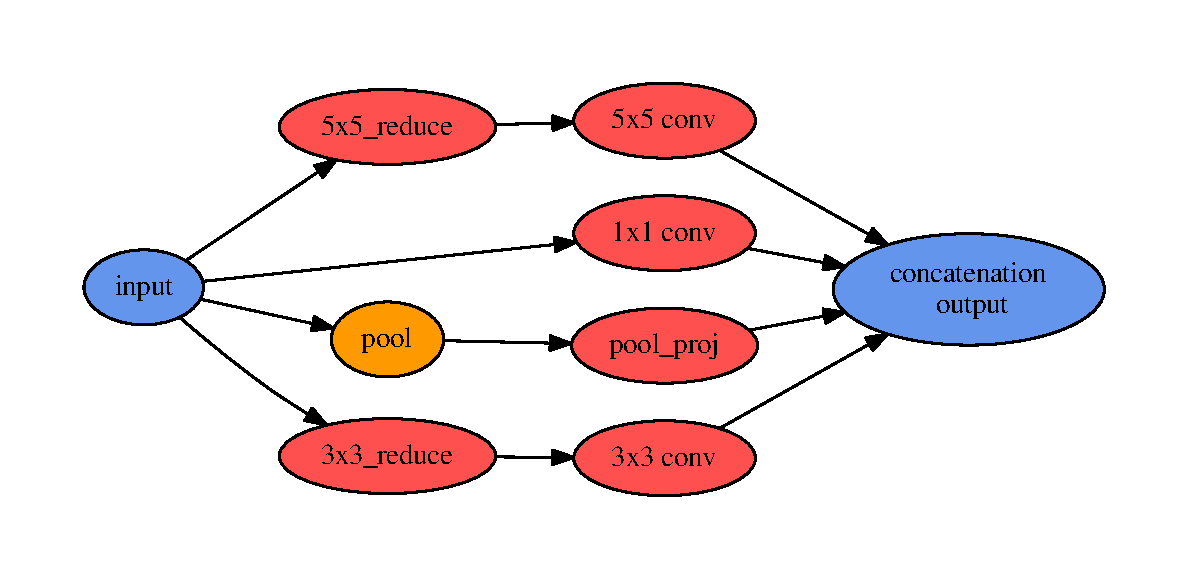
\includegraphics[scale=.45]{fig/inception.pdf}\\
  \caption{Inception Cell. $n\times n$ stands for size $n$ receptive field, $n\times n\_reduce$ stands for the $1\times 1$ convolutional layer before the $n\times n$ convolution layer and $pool\_proj$ is another $1\times 1$ convolutional layer after the MAX pooling layer. The output layer concatenate all its input layers.}\label{incept}
\end{figure}

\subsection{Food Datasets}
Besides ImageNet dataset, there are many popular benchmark datasets for image classification tasks such as Caltech dataset and CIFAR dataset, which contain hundreds of classes. However, in this paper, we try to focus on a more specific area, food classification. Compared to other classification tasks, there are some properties of the food (dishes) which make the tasks become a real challenge:
i)food doesn't have any distinctive spatial layout: for other tasks like scene recognition, we can always find some discriminative features such as buildings or trees, etc.
ii) food class is a small sub-category among all the categories in daily life, so the inter-class variation is relatively small; on the other hand, the contour of a food varies depending on many aspects such as the point of the view or even its component.
So these properties make food classification catastrophic for some recognition algorithms. Therefore, the training these two models on food classification task can reveal some important aspects of themselves and help us better understand their architectures. In this paper, we used two image datasets Food256 \cite{kawano14c}\footnote{Dataset can be found http://foodcam.mobi/dataset.html} and Food101 \cite{bossard14}\footnote{Dataset can be found http://www.vision.ee.ethz.ch/datasets\_extra/food-101}. It is worthy to mention that PFID dataset is also a big public image database for classification, but their images are collected in a laboratory condition which is considerably not applicable for real recognition task.

\textbf{Food-256 Dataset.}
This is a relatively small dataset containing 256 kinds of foods and 31644 images from various countries such as French, Italian, US, Chinese, Thai, Vietnamese, Japanese and Indonesia. The distribution among classes is not even and the biggest class (vegetable tempura) contains 731 images while the smallest one contains just 100 images. For this "small" dataset, we randomly split the data into training and testing set, using around 80\% (25361 images) and 20\%(6303 images) of the original data respectively and keep the class distribution in these two sets uniform. The collector of this dataset also provides boundary box for each image to separate different foods and our dataset is cropped according to these boundary boxes.

\textbf{Food-101 Dataset.}
This dataset contains 101-class real-world food (dish) images which were taken and labeled manually. The total number of images is 101,000 and there are exactly 1000 images for each of the class. Also, each class has been divided into training and testing set containing 750 images and 250 images respectively by its collector. The testing set is well cleaned manually while the training set is not well cleaned on purpose. This noisy training set is more similar to our real recognition situation and it is also a good way to see the effect of the noise on these two architectures.

Data argumentation is an efficient way to enrich the data. There are also some techniques that can applied to enlarge the dataset such as subsampling and mirroring. The original images are firstly resized to $256\times 256$ pixels. We crop the 4 corners and center for each image according to the input size of each model and flap the 5 cropped images to obtain 10 crops. For the testing set, the prediction of an image is the average prediction of the 10 crops.
